% !TeX program = xelatex
\documentclass{anisyan-resume}

%--------------------
%      Packages
%--------------------
\usepackage[utf8]{inputenc}
\usepackage{adjustbox}
\usepackage{amssymb}
\usepackage{graphicx}
\usepackage{caption}
\usepackage{subcaption}
\usepackage{array}
\usepackage{makecell}
\usepackage[top=5mm,
	bottom=5mm,
	left=5mm,
	right=10mm]{geometry}
\usepackage{fontawesome}
\usepackage{xcolor}
\usepackage{setspace}
\usepackage[colorlinks = true,
	linkcolor = blue,
	urlcolor  = blue,
	citecolor = blue,
	anchorcolor = blue]{hyperref}
\usepackage{multirow}
\usepackage{tabularx}
\usepackage{enumitem}
\usepackage{fontspec}
\setmainfont{Arial}

\begin{document}
	%--------------------
	%      HEADER
	%--------------------
	\begin{tabular}{ m{4cm} m{9.5cm} m{4.7cm} }
		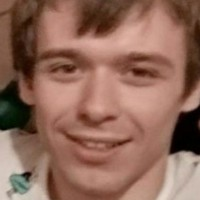
\includegraphics[width=4cm, height=4cm]{avatar.jpeg}
		&
		\begin{tabular}{ p{9.5cm} }
			\textbf{\Huge Alexander Anisimov} \\
			\Large {System/Embedded Software Engineer} \\
			\vspace{1pt}
			\large{1 year as TrustZone Software Developer,} \\
			\large{3 years as Embedded Software Developer.} \\
			\vspace{2pt}
			\large{Looking for an Embedded Linux} \\
			\large{or System Software related position.}	
		\end{tabular}
		&
		\makepersonallinks{79175190834}
		 					{+7(917)-519-08-34}
		 					{anisimov.alexander.s}
		 					{https://github.com/anisyanka}
		 					{https://www.linkedin.com/in/anisyanka/}
		 					{https://stackoverflow.com/users/9308555/anisyanka}
	\end{tabular}

	%--------------------
	%      SKILLS
	%--------------------
	\vspace{10pt}
	\section{\textbf{SKILLS}}
	\vspace{10pt}
	\def\arraystretch{1.2}
	\begin{tabular}{ >{\quad}l p{9.5cm} }
		\normalsize\textbf{Basis} & \normalsize{C, Bash, GNU make, Git} \\
		\normalsize\textbf{Have experience with} & \normalsize{C++, QML, Python} \\
		\normalsize\textbf{Other} & \normalsize{Vim, Markdown, \LaTeX, RPM spec} \\
		\normalsize\textbf{Keywords} & \normalsize{ARM, TrustZone, REE, TEE, Linux kernel, LDD, hypervisors, microcontrollers, bootloaders} \\
	\end{tabular}

	%--------------------
	%      EDUCATION
	%--------------------
	\section{\textbf{EDUCATION}}
	\vspace{10pt}
	\def\arraystretch{1.2}
	\begin{tabular}{ m{12cm} }
		\quad\href{https://eng.mephi.ru/}{\large \textbf{National Research Nuclear University MEPhI}} \\
		\vspace{5pt}
		\quad\normalsize{Bachelor's degree, nuclear physics, sept. 2013 - june 2017} \\
		\quad\normalsize{Master's degree, embedded systems, sept. 2017 - june 2019} \\
	\end{tabular}

	%--------------------
	%      WORK EXPERIENCEE
	%--------------------
	\vspace{5pt}
	\section{\textbf{WORK EXPERIENCE}}
	\vspace{10pt}
	\renewcommand\arraystretch{0.5}
	\begin{tabularx}{\textwidth}{>{\quad}p{4cm} |@{\timelinebullet} l}
		% OMP
		%-------------------------------------------------------------------------------------------
		\normalsize\textbf{Jul 2019 -- now}
		&
		\renewcommand\arraystretch{1}
		\begin{tabular}[t]{ p{15cm} }
			\large{\textbf{System Software Engineer}} \texttt{\textbf{@}}\href{https://sailfishos.org/}{\textbf{Open Mobile Platform}} \\
			\normalsize{Mobile OS based on Linux}
			\renewcommand\labelitemi{{\boldmath$\cdot$}}
			\begin{itemize}[noitemsep, topsep=5pt, parsep=0pt, partopsep=0pt]
				\item {\small Development TEE side of Russian fork of Sailfish OS (Aurora OS)}
				\item {\small Development hardware-backed keystore and trusted services}
				\item {\small Designed new features for Linux kernel OP-TEE driver for in-house Linux distro}
				\item {\small CVE fixing for government certification (FSTEK Russia)}
				\item {\small Took part in preparation solution for sharing hardware resources between REE and TEE worlds}
			\end{itemize}
		\end{tabular} \\

		% Yandex
		%-------------------------------------------------------------------------------------------
		\normalsize\textbf{Sept 2019 -- Mar 2019}
		&
		\renewcommand\arraystretch{1}
		\begin{tabular}[t]{ p{15cm} }
			\large{\textbf{Embedded Software Engineer}} \texttt{\textbf{@}}\href{https://en.wikipedia.org/wiki/Yandex}{\textbf{Yandex}}\\
			\normalsize{Self-driving cars}
			\renewcommand\labelitemi{{\boldmath$\cdot$}}
			\begin{itemize}[noitemsep, topsep=5pt, parsep=0pt, partopsep=0pt]
				\item {\small Development emergency stop button for self-driving cars (FreeRTOS, STM32, CAN, radio module)}
				\item {\small Reverse engineering for update protocol for radio modules to update its firmware by other chip}
				\item {\small Development from scratch driver for SPI-based e-paper displays}
				\item {\small Writing unit-tests with cpputest for one of main board in car}
			\end{itemize}
		\end{tabular} \\

		% SmartAirkey
		%-------------------------------------------------------------------------------------------
		\normalsize\textbf{Feb 2018 -- Sept 2018}
		&
		\renewcommand\arraystretch{1}
		\begin{tabular}[t]{ p{15cm} }
			\large{\textbf{Embedded Software Engineer}} \texttt{\textbf{@}}\href{https://smartairkey.com/en/}{\textbf{SmartAirkey}}\\
			\normalsize{Wireless solutions startup}
			\renewcommand\labelitemi{{\boldmath$\cdot$}}
			\begin{itemize}[noitemsep, topsep=5pt, parsep=0pt, partopsep=0pt]
				\item {\small Development firmware for a Bluetooth-lock based on Nordic BLE stack and FreeRTOS}
				\item {\small Development user-space Linux driver to control the lock over UART}
				\item {\small Soldering and testing boards}
			\end{itemize}
		\end{tabular} \\

		% Amplituda
		%-------------------------------------------------------------------------------------------
		\normalsize\textbf{Sept 2016 -- Feb 2018}
		&
		\renewcommand\arraystretch{1}
		\begin{tabular}[t]{ p{15cm} }
			\large{\textbf{Junior Embedded Engineer}} \texttt{\textbf{@}}\href{http://www.amplituda.ru/}{\textbf{Amplituda}}\\
			\normalsize{Radiation safety technologies}
			\renewcommand\labelitemi{{\boldmath$\cdot$}}
			\begin{itemize}[noitemsep, topsep=5pt, parsep=0pt, partopsep=0pt]
				\item {\small Development firmware for $\gamma$-sensors based on RS-485 and stm32f103}
				\item {\small Development USB CDC devices to connect its to PC-apps}
				\item {\small Development low-level drivers for ADC, DAC, OLED-controllers, touchscreen, RTC, DHT11, HD44780 and so on}
			\end{itemize}
		\end{tabular}
	\end{tabularx}

	%--------------------
	%      ACHIEVEMENTS
	%--------------------
	\section{\textbf{ACHIEVEMENTS}}
	\vspace{10pt}
	\renewcommand\labelitemi{{\boldmath$\cdot$}}
	\begin{itemize}[noitemsep, topsep=0pt, parsep=0pt, partopsep=0pt]
		\item \small{Fixed CVE-2020-6096 in GNU C Library for ARMv7 memcpy()} \\
			\href{https://sourceware.org/pipermail/libc-alpha/2020-June/114702.html}{https://sourceware.org/pipermail/libc-alpha/2020-June/114702.html};\\
			\href{https://sourceware.org/pipermail/libc-alpha/2020-June/114919.html}{https://sourceware.org/pipermail/libc-alpha/2020-June/114919.html};\\
			\href{https://sourceware.org/pipermail/libc-alpha/2020-July/115923.html}{https://sourceware.org/pipermail/libc-alpha/2020-July/115923.html};\\
			\href{https://sourceware.org/pipermail/libc-alpha/2020-July/115924.html}{https://sourceware.org/pipermail/libc-alpha/2020-July/115924.html};
	\end{itemize}
\end{document}

